% Chapter Template

\chapter{Data Analysis and Methods} % Main chapter title

\label{Chapter:Data} 

%----------------------------------------------------------------------------------------

%----------------------------------------------------------------------------------------
wohin damit? \\ \\
PHA pro Spin...
Ideal / mit Fehlern alpha, beta


SWICS provides two types of data products from the analogue signals Tof, ESSD and the EPQ-Step.
24-bit



\section{Data products}
PHA words, data transmission

\subsection{Priority weighting}
SWICS performs an on-board mass and mass-per-charge-classification. For every ion with valid measurements the $m$ and $mpq$ are calculated based on the measurements of ESSD, Tof and the particle's EPQ-step using a look-up-table technique.\\
On the one hand these values are used for sorting the ions into predefined boxes in the m-mpq-space which yield in the so-called matrix rate, a second data product that is provided by SWICS.\\
Secondly, and more important for our analysis, the m and mpq information is used to sort every measured ion into one of three priority ranges.

Range, BRW\\ \\
\begin{tabular}{c|c|c}
	%\hline
	Range 0 & $m < 8.7$;  $m_0 : mpq < 3.3$ & $\mathrm{H}$, $\mathrm{He^+}$, $\mathrm{He^{2+}}$; Doubles\\ 
	\hline 
	Range 1 & $m > 8.7$ & Heavier ions \\ 
	\hline 
	Range 2 & $m_0 : mpq > 3.3$ & Doubles \\ 
	%\hline 
\end{tabular} 

\subsection{Detection efficiencies}
Threshold, Doubles...



%
%
%

\section{ET matrices, identification}
Fig. \ref{fig:et_matrix} shows longterm PHA data collected with Ulysses SWICS over two years for EPQ Step 25 (= Energy per charge TODO). For every particle with valid measurements the $\mathrm{E_{SSD}}$ channel is plotted over the ToF channel. As a particle's mass and mass-per-charge is connected to the measured values $EpQ$, $\tau$ and $E_{SSD}$ by equations \ref{eq:swics_set1} --  \ref{eq:swics_set3}, every ion species occupies a distinct position in the so-called \textit{ET-Matrix}.


\begin{figure}[h]
	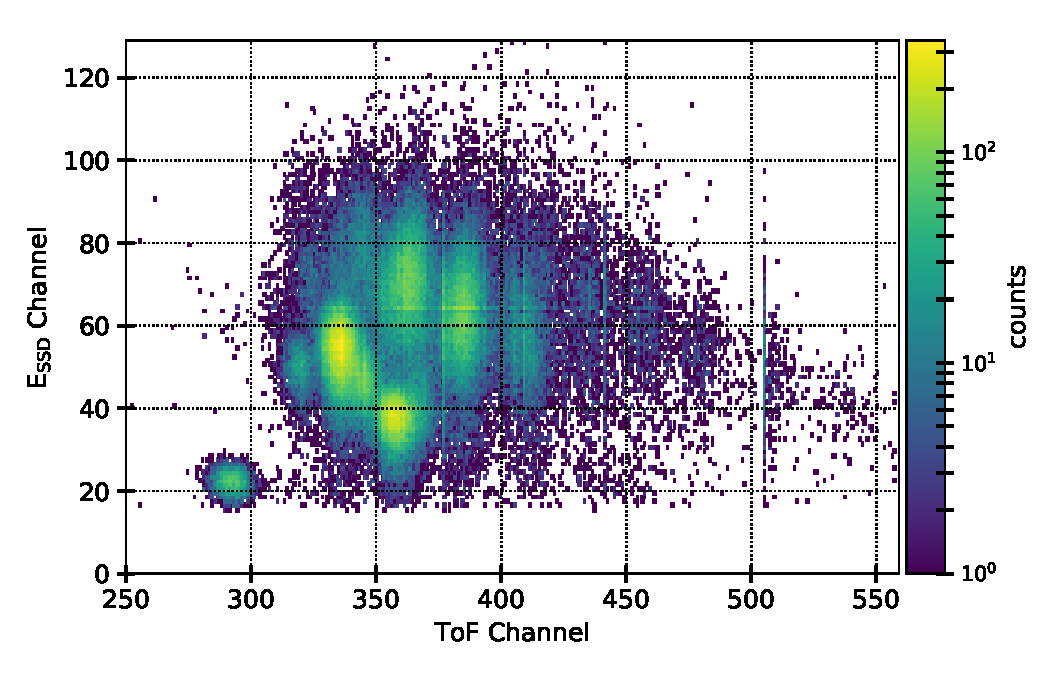
\includegraphics[width=0.9\textwidth]{Figures/et_matrix.pdf}
	\centering
	\caption{test}
	\label{fig:et_matrix}
\end{figure}


\section{Filter He+}

\begin{figure}[h]
	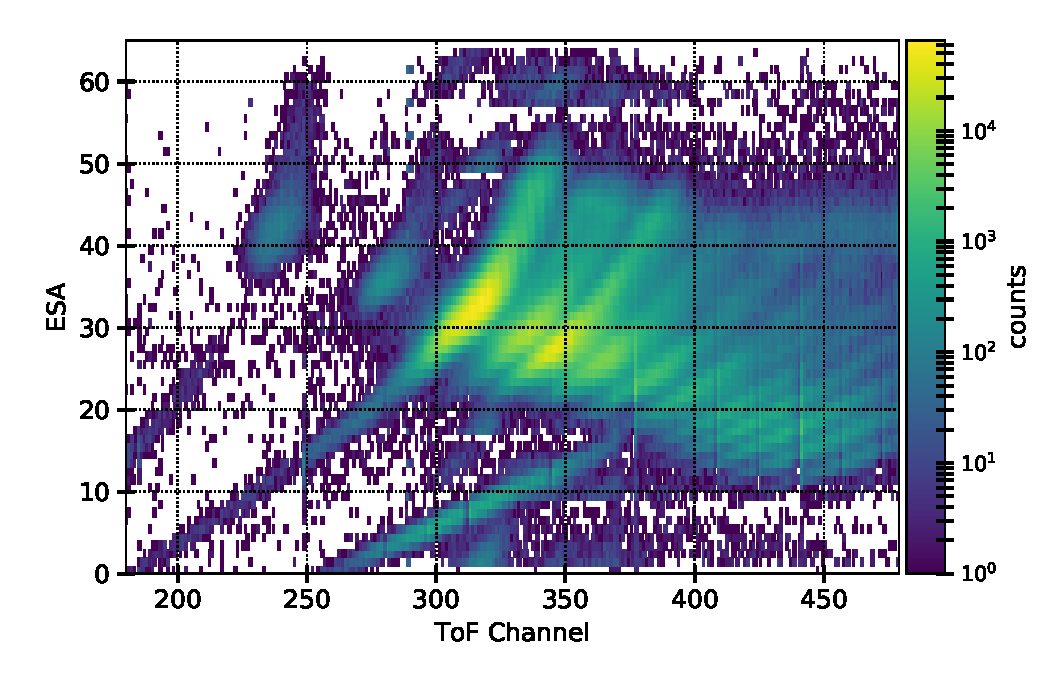
\includegraphics[width=0.9\textwidth]{Figures/epq_all.pdf}
	\centering
	\caption{test}
	\label{fig:epq_all}
\end{figure}


For extracting only the $\mathrm{He^+}$ events from the PHA data we plot the events' energy-per-charge over their measured ToF.
Teilchen derselben mpq werden auf Kurven $todo$ geortet. Spezies höherer Mpq finden sich auf Kurven mit größeren ToF-Werten. Man kann so z.B. todo, todo und todo identifizieren. Unten ist He gut zu erkennen weil suprathermal. An die suprathermalen $He$-Teilchen schließen sich zu höheren ToF andere Teilchen mit derselben mpq auf der gleichen Kurve an. Weil die Kurven dort enger liegen, kann man He in dem Bereich auch nicht von anderen mit ähnlicher mpq unterscheiden.
We can take advantage of SWICS' on-board priority weighting. We only plot the Range0-events. This roughly cuts out events with $m>8.7$. Nur H, He2+, He+ bleiben übrig als prominente Ionen. Man sieht, dass auch einige schwerere in die Box reinlecken, aber das betrifft nicht die ESA-Steps, in denen Helium auftritt.\\
Man kann jetzt prima per Auge eine Maske legen. Zusätzlich w filtern um eventullen Hintergrund zu unterdrücken...?
Man sieht, dass wir nur Helium-PHAs bis EpQ-Step todo auswerten. Der Grund ist, dass He1+ aufgrund der geringen Masse nicht genug Energie hat, die Triggerschwelle des SSDs zu überschreiten. Somit liegen He1+-Ionen bei höheren ESA-Steps (kleineren Energien pro Ladung) als Double Coincidences vor und taugen nicht für unsere Analyse.
\\
Für alle Jahre. Anzahl: todo


\section{Filter He2+}
für die spätere Kalibrierung (todo: Verweis) brauchen wir eine Spezies, bei der wir davon ausgehen, dass sie sich mit dem SW-Bulk bewegt und die als Triple Coinzidences vorliegt (für die Richtungsinformation). We choose He2+ wegen guter Statistik und auch in Range0. Im Gegensatz zu He1+ auch bei höheren ESA-Steps anzutreffen, weil mehr Nachbeschleunigung durch die höhere Ladung. Dadurch nicht so schnell unter SSD-Threshold. Gleiches Verfahren, einfach ausschneiden. Hier ist es nicht so wichtig, alles mitzubekommen, weil wir anhand von He2+ keine Analyse der VDF durchführen wollen. 
\\
Für alle Jahre. Anzahl: todo
\\ \\
Weitere Daten: vsw von SWOOPS, B-Feld




\section{Collimator}

Geometrie, Aspect Angle: Ausrichtung zu jedem Zeitpunkt bekannt
(FoV) (hierher die Kalibration! Nur damit funktioniert die Ausrichtung)
Wir füllen die einzelnen Bereiche mit verschiedenen möglichen Messpunkten

Übergang FoV -> vSpace:
Richtungsinfo aus FoV
Betrag aus EpQ-Steps
außerdem: Eigengeschwindigkeit Ulysses

Dann nehmen wir PHA-Worte und können jedem ein gemessenes Volumen im Phasenraum zuordnen (?).


\section{Phasenraumbla}
Mittlere Phasenraumdichte in einem Bin, in den zwei Instrumentenbins A und B reingehen:

\begin{align}
\bar{\rho} = \frac{N_A + N_B}{\frac{N_A}{N_{A,ges}} V_A + \frac{N_B}{N_{B,ges}} V_B }
\end{align}

Dabei ist $N_i$ die Anzahl der Hits, die im Messbin gelandet sind und $N_{i,ges}$ die gesamte Anzahl an Bins. Hits heißt GEsamtcounts durch Detektoranzahl. Eigentlich gebe ich statt $N_i$ $N_i \cdot Detektoranzahl$ rein, aber das kürzt sich ja raus.\\ \\
Effizienz und Sektorgewichte dazu:\\
Allg.:
\begin{align*}
\rho = \frac{N \cdot brw}{V \cdot Eff}
\end{align*}
Und dann
\begin{align}
\bar{\rho} = \frac{N_A + N_B}{\frac{N_A}{N_{A,ges}} \frac{V_A \cdot eff_A}{brw_A} + \frac{N_B}{N_{B,ges}} \frac{V_B \cdot eff_B}{brw_B} }
\end{align}


